%
% rieszbeispiel.tex -- slide template
%
% (c) 2021 Prof Dr Andreas Müller, OST Ostschweizer Fachhochschule
%
\bgroup
\begin{frame}[t]
\setlength{\abovedisplayskip}{5pt}
\setlength{\belowdisplayskip}{5pt}
\frametitle{Linearform auf $L^2$-Funktionen}
\vspace{-20pt}
\begin{columns}[t,onlytextwidth]
\begin{column}{0.48\textwidth}
\begin{block}{Linearform auf $\mathbb{C}^n$}
\begin{align*}
{\color{blue}x}&=\begin{pmatrix}x_1\\x_2\\\vdots\\x_n\end{pmatrix},
&
f({\color{blue}x})
&= 
\begin{pmatrix}f_1&f_2&\dots&f_n\end{pmatrix} {\color{blue}x}
\\
\uncover<2->{
{\color{red}v}&=
\rlap{$
\begin{pmatrix}
\overline{f}_1&\overline{f}_2&\dots&\overline{f}_n
\end{pmatrix}^t
\uncover<3->{\;\Rightarrow\;
f({\color{blue}x})=\langle {\color{red}v},{\color{blue}x}\rangle}
$}}
\end{align*}
\end{block}
\end{column}
\begin{column}{0.48\textwidth}
\uncover<4->{%
\begin{block}{Linearform auf $L^2([a,b])$}
\begin{align*}
{\color{red}x}&\in L^2([a,b])
\\
\uncover<5->{
f&\colon L^2([a,b]) \to \mathbb{C}
: {\color{red}x} \mapsto f({\color{red}x})}
\intertext{\uncover<6->{Riesz-Darstellungssatz: $\exists {\color{blue}v}\in L^2([a,b])$}}
\uncover<7->{f({\color{red}x})
&=
\int_a^b {\color{blue}\overline{v}(t)}{\color{red}x(t)}\,dt}
\end{align*}
\end{block}}
\end{column}
\end{columns}
\begin{center}
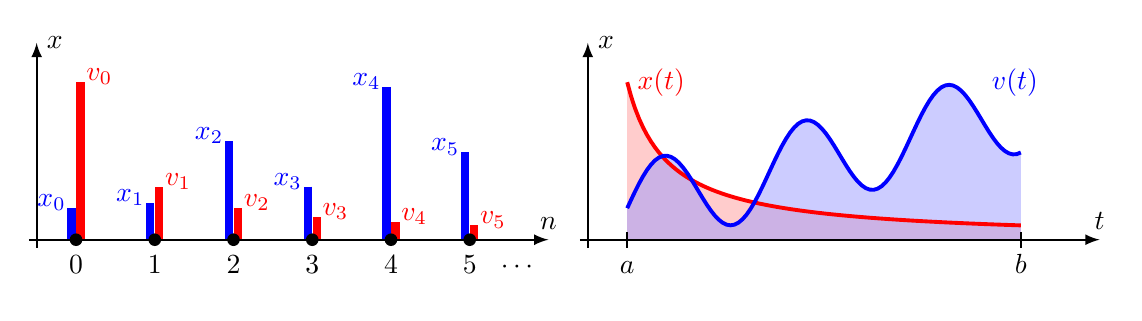
\begin{tikzpicture}[>=latex,thick]
\begin{scope}[xshift=-3.5cm]
\def\s{0.058}
\foreach \n in {0,...,5}{
\uncover<3->{
	\draw[color=red,line width=3pt]
		({\n+\s},{1/(\n+0.5)}) -- ({\n+\s},0);
	\node[color=red] at ({\n},{-0.2+1/(\n+0.5)})
		[above right] {$v_\n\mathstrut$};
}
	\draw[color=blue,line width=3pt]
		({\n-\s},{0.4+0.55*sin(200*\n)+0.25*\n}) -- ({\n-\s},0);
	\node[color=blue] at ({\n},{-0.2+0.4+0.55*sin(200*\n)+0.25*\n})
		[above left] {$x_\n\mathstrut$};
}
\draw[->] (-0.6,0) -- (6,0) coordinate[label={$n$}];
\draw[->] (-0.5,-0.1) -- (-0.5,2.5) coordinate[label={right:$x$}];
\foreach \n in {0,...,5}{
	\fill (\n,0) circle[radius=0.08];
	\node at (\n,0) [below] {$\n$\strut};
}
\node at (5.6,0) [below] {$\cdots$\strut};
\end{scope}
\uncover<4->{
\begin{scope}[xshift=3.5cm]
\uncover<7->{
\fill[color=red!40,opacity=0.5] 
	plot[domain=0:5,samples=100] (\x,{1/(\x+0.5)})
	--
	(5,0) -- (0,0) -- cycle;
}
\fill[color=blue!40,opacity=0.5]
	plot[domain=0:5,samples=100] (\x,{0.4+0.55*sin(200*\x)+0.25*\x})
	-- (5,0) -- (0,0) -- cycle;
\uncover<7->{
\draw[color=red,line width=1.4pt]
	plot[domain=0:5,samples=100] (\x,{1/(\x+0.5)});
\node[color=red] at (0,2) [right] {$x(t)$};
}

\draw[color=blue,line width=1.4pt]
	plot[domain=0:5,samples=100] (\x,{0.4+0.55*sin(200*\x)+0.25*\x});
\node[color=blue] at (4.5,2) [right]{$v(t)$};

\draw[->] (-0.6,0) -- (6.0,0) coordinate[label={$t$}];
\draw[->] (-0.5,-0.1) -- (-0.5,2.5) coordinate[label={right:$x$}];
\draw (0.0,-0.1) -- (0.0,0.1);
\node at (0.0,0) [below] {$a$\strut};
\draw (5.0,-0.1) -- (5.0,0.1);
\node at (5.0,0) [below] {$b$\strut};
\end{scope}
}
\end{tikzpicture}
\end{center}
\end{frame}
\egroup
